\documentclass[t]{beamer}

%\documentclass[handout, t]{beamer}
\setbeamertemplate{navigation symbols}{}
\usepackage{pstricks}
\usepackage{mathtools}
\usepackage{amsfonts}
\usepackage{mathrsfs}
\usepackage{amsmath}
\setbeamertemplate{navigation symbols}{}
\usepackage{bm}
\usepackage[UTF8]{ctex}
\usetheme{AnnArbor}
\usefonttheme{serif}
\useinnertheme{rounded}
\usecolortheme{dolphin}
\setbeamertemplate{blocks}[rounded][shadow=true]

\newcommand{\dif}{{\;\rm d}}
\usepackage{graphicx}
\usepackage{pgf}
\usepackage{tikz}
\usetikzlibrary{arrows, decorations.pathmorphing, backgrounds, positioning, fit, petri, automata}
\tikzset{>=stealth}

\usepackage{setspace}
\setmainfont{Times New Roman}
\setCJKmainfont{Microsoft YaHei}


\hypersetup{pdfpagemode=FullScreen}
\renewcommand{\Pr}{\mathbb{P}}
\usepackage{blkarray}


\setbeamercolor{block title}{bg=red!10!white}
\setbeamercolor{block body}{bg=gray!10!white}

\usepackage{multicol}
\newcommand{\E}{\mathbb{E}}
\newcommand{\EP}{\mathbb{E}^{\mathbb{P}}}
\newcommand{\EQ}{\mathbb{E}^{\mathbb{Q}}}
\newcommand{\Var}{{\rm Var}}
\newcommand{\Cov}{{\rm Cov}}


\begin{document}
\fontsize{11}{18}\selectfont


\CTEXindent



  \title{第十二章~~期权定价的离散模型}
\author{随机过程及其在金融中的应用}
\date{中国人民大学出版社}
  \begin{frame}
    \maketitle
  \end{frame}

\begin{frame}{引言}
	期权定价的离散模型中最为著名的就是考克斯、罗斯和鲁宾斯坦(Cox,Ross,Rubinstein,1979)提出的二项式模型(binomial model)。
	\begin{center}
\begin{tabular}{ccc}
\includegraphics[height=0.4\textheight]{fig/Cox.jpeg}
& \includegraphics[height=0.4\textheight]{fig/Ross.jpg}& \includegraphics[height=0.4\textheight]{fig/Rubin.jpg}\\
约翰·考克斯 & 斯蒂芬·罗斯 & 马克·鲁宾斯坦\\
(1943---\;) &  (1944---2017)   &  (1944---2019)\\
\end{tabular}
	\end{center}
\end{frame}



\begin{frame}{本章内容}
\tableofcontents

\end{frame}

\section{单期二项式模型}
\begin{frame}{单期二项式模型}
	单期二项式模型(single period binomial model),是指初始时刻为$t=0$,结束时刻在$t=1$,并且在未来时刻$1$,股票(即标的资产)的价格只有两种可能状态的模型。
	
	为了叙述方便,假设股票的价格为$S$,对应的期权价格为$V$;初始时刻两者的价格分别为$S(0)$和$V(0)$,未来到期时刻的价格分别为$S(1)$和$V(1)$
。

\end{frame}


\begin{frame}{单期二项式模型(cont.)}
考虑到股票未来价格的涨跌,股价上涨(up)和下跌(down)分别记作$S_u(1)$和$S_d(1)$;两种情形下期权的价格分别记作$V_u(1)$和$V_d(1)$。
\begin{center}
	\begin{tikzpicture}[>=stealth, thick, scale=.8]
		\node (A) at (0,0) {$S(0)$};
		\node (B) at (2.5,1) {$S_u(1)$};
		\node (C) at (2.5,-1) {$S_d(1)$};
		\draw [->](A)--(B); \draw [->](A)--(C);
		\node at (0,-1.8){$t=0$};
		\node at (2.5,-1.8){$t=1$};
		
		\node at (1.5, -2.5) {(a)股票的二叉树};
		\end{tikzpicture}\qquad \qquad
		\begin{tikzpicture}[>=stealth, thick, scale=.8]
		\node (A1) at (0,0) {$V(0)$};
		\node (B1) at (2.5,1) {$V_u(1)$};
		\node (C1) at (2.5,-1) {$V_d(1)$};
		\draw [->](A1)--(B1); \draw [->](A1)--(C1);
		\node at (0,-1.8){$t=0$};
		\node at (2.5,-1.8){$t=1$};
		\node at (1.5, -2.5){(b)期权的二叉树};
		\end{tikzpicture}
\end{center}

构造一个组合,其在初始时刻的总价值为$X(0)$,假设采用自融资策略,购买了
$\Delta(0)$股的股票,并将剩余资金全部用于购买一份期权。
\end{frame}


\begin{frame}{单期二项式模型(cont.)}
该组合在当前时刻的价值为:
\begin{equation*}
X(0)=\Delta(0) S(0)+V(0)
\end{equation*}
在未来时刻$1$,该组合的可能价值分别为:
\begin{align*}
X_u(1)&= \Delta(0) S_u(1)+V_u(1) \\
X_d(1)&= \Delta(0) S_d(1)+V_d(1) 
\end{align*}
我们希望得到满足条件的$\Delta(0)$和$V(0)$,使得在未来时刻$1$,组合的价值保持不变,即满足$X_u(1)=X_d(1)$。
\end{frame}


\begin{frame}{单期二项式模型(cont.)}
根据前面的定理可知:对于这种组合价值不变的资产,在无套利条件下,其当前的价值$X(0)$与未来时刻的价值$X(1)$之间的关系式如下:
\[X(1)=X(0)(1+r)\]
综合上面各式,可以得到:
\begin{align}
X(0)(1+r)&= \Delta(0) S_u(1)+V_u(1) \label{bino-1}\\
X(0)(1+r)&= \Delta(0) S_d(1)+V_d(1) \label{bino-2}
\end{align}
取$0<q<1$,并对式(\ref{bino-1})两端同乘以$q$,对式(\ref{bino-2})两端同乘以$(1-q)$,并将两式相加可得:
\begin{equation*}
    \begin{split}
        X(0)(1+r)&=\Delta(0) \Big[qS_u(1)+(1-q)S_d(1) \Big]+\Big[qV_u(1)+(1-q)V_d(1) \Big]
    \end{split}
\end{equation*}
\end{frame}

\begin{frame}{单期二项式模型(cont.)}\small
	将$X(0)=\Delta(0) S(0)+V(0)
	$代入可得:
	\begin{equation*}
		\begin{split}
			&\Delta(0)\Big[ {q{S_u}(1) + (1 - q){S_d}(1) - {S(0)}  (1+r)} \Big] \\
			&= {V(0)}  {(1+r)} - \Big[ {q{V_u}(1) + (1 - q){V_d}(1)} \Big]    
		\end{split}
	\end{equation*}
	若令上式的左右两侧均等于零,则有:
	\begin{equation*}
	\begin{cases}
		\vspace{1ex}		q{S_u}(1) + (1 - q){S_d}(1) - {S(0)}  (1+r)=0\\
	{V(0)}  {(1+r)} - \big[ {q{V_u}(1) + (1 - q){V_d}(1)} \big]=0
	\end{cases}
	\end{equation*}
	最终可得:
	\begin{equation*}
	\begin{cases}
\vspace{1ex}	S(0)=\dfrac{q{S_u}(1) + (1 - q){S_d}(1)}{1+r}\\
	V(0)=\dfrac{q{V_u}(1) + (1 - q){V_d}(1)}{1+r}
	\end{cases}
	\end{equation*}

\end{frame}

\begin{frame}{“概率”}
如果将$q$看成一个概率的话,则当前股票的价格$S(0)$可以看作未来股票价格期望值的贴现;类似地,当前期权的价格$V(0)$也可以看作期权未来可能价格期望值的贴现。	
	\begin{equation*}
		\begin{cases}
	\vspace{1ex}	S(0)=\dfrac{q{S_u}(1) + (1 - q){S_d}(1)}{1+r}\\
		V(0)=\dfrac{q{V_u}(1) + (1 - q){V_d}(1)}{1+r}
		\end{cases}
		\end{equation*}
				
\begin{center}\small
	\begin{tikzpicture}[>=stealth, thick,scale=.8]
		\node (A) at (0,0) {$S(0)$};
		\node (B) at (2.5,1) {$S_u(1)$};
		\node (C) at (2.5,-1) {$S_d(1)$};
		\draw [->](A)  to (B)  ; \draw [->](A)--(C);
		\node at (1,.8){$q$};  \node at (1,-.8){$(1-q)$};  
		\node at (0,-1.8){$t=0$};
		\node at (2.5,-1.8){$t=1$};
		
		\node at (1.5, -2.5) {(a)股票的二叉树};
		\end{tikzpicture}\qquad 
		\begin{tikzpicture}[>=stealth, thick,scale=.8]
		\node (A1) at (0,0) {$V(0)$};
		\node (B1) at (2.5,1) {$V_u(1)$};
		\node (C1) at (2.5,-1) {$V_d(1)$};
		\draw [->](A1)--(B1); \draw [->](A1)--(C1);
		\node at (1.2,.8){$q$};  \node at (1.2,-.8){$(1-q)$};  
		\node at (0,-1.8){$t=0$};
		\node at (2.5,-1.8){$t=1$};
		\node at (1.5, -2.5){(b)期权的二叉树};
		\end{tikzpicture}
\end{center}
\end{frame}

\begin{frame}{风险中性概率}
	需要说明的是,这里的概率$q$并不是真实市场上的概率,而是我们在推导过程中人为构造的概率,称为风险中性概率(risk-neutral probability)。

	将这种由风险中性概率所组成的概率测度称作风险中性测度(risk-neutral measure),记作$\mathbb{Q}$。
	
	为了区分,真实市场上资产价格变动的概率记作$p$,相应的概率测度记作$\mathbb{P}$。这样的两个概率测度是等价的(equivalent),记作$\mathbb{P}\sim \mathbb{Q}$。
\end{frame}

\begin{frame}{等价测度的定义}
	在同一个样本空间$S$内的两个概率测度$\mathbb{P}$和$\mathbb{Q}$,若对$S$中的任意子样本空间$A$,均有以下充要条件成立:
\[\mathbb{P}(A)=0\Longleftrightarrow \mathbb{Q}(A)=0 \]
或者
\[\mathbb{P}(A)\ne 0\Longleftrightarrow \mathbb{Q}(A)\ne 0 \]
则称$\mathbb{P}$和$\mathbb{Q}$是等价测度(equivalent measure),记作$\mathbb{P}\sim \mathbb{Q}$。
\begin{block}{}
	两个概率测度等价,则意味着事件$A$在测度$\mathbb{P}$下有可能发生,相应地在测度$\mathbb{Q}$下也有可能发生;反之亦然。
\end{block}

\end{frame}

\begin{frame}{风险中性概率的表达式}
	如果进一步假设未来时刻股票价格上涨的倍数为$u$,下跌的倍数为$d$,并且$0<d<1<u$,则有:
	  \begin{equation*}
S_u(1)=u\cdot S(0),\qquad S_d(1)=d\cdot S(0)
\end{equation*}
将上式代入$S(0)=\dfrac{q{S_u}(1) + (1 - q){S_d}(1)}{1+r}$,最终可得:
\begin{equation*}
q=\frac{(1+r)-d}{u-d}
\end{equation*}
由此可见,风险中性概率$q$只与无风险利率$r$、期限$t=1$、上涨倍数$u$ 和下跌倍数$d$有关,而与股票的价格$S(0)$无关。
\end{frame}

\begin{frame}{例题1:看涨期权}
	一只股票的当前价格为20元,3个月后股价有可能涨至22元,也有可能跌至18元。3个月后到期的该股票看涨期权的行权价为21元,假设无风险利率为4\%。

问:该看涨期权的当前价格应为多少?
\end{frame}

\begin{frame}{解答}
	首先,根据题目中的条件可得:$$u=\frac{22}{20}=1.1,\quad d=\frac{18}{20}=0.9$$
相应的股票和期权的二叉树如下所示:
\begin{center}
	\begin{tikzpicture}[>=stealth, thick, scale=.8]
	\node (A) at (0,0) {$20$};
	\node (B) at (2.5,1) {$22$};
	\node (C) at (2.5,-1) {$18$};
	\draw [->](A)  to (B)  ; \draw [->](A)--(C);
	\node at (1,.8){$q$};  \node at (1,-.8){$(1-q)$};  
	%\node at (0,-1.8){$t=0$};
	%\node at (2.5,-1.8){$t=1$};
	
	\node at (1.5, -1.8) {(a)股票的二叉树};
	\end{tikzpicture}\qquad 
	\begin{tikzpicture}[>=stealth, thick,scale=0.8]
	\node (A1) at (0,0) {$V(0)$};
	\node (B1) at (2,1) [right]{$\max(0, 22-21)=1$};
	\node (C1) at (2,-1) [right]{$\max(0, 18-21)=0$};
	\draw [->](A1)--(B1); \draw [->](A1)--(C1);
	\node at (1.2,.8){$q$};  \node at (1.2,-.8){$(1-q)$};  
	%\node at (0,-1.8){$t=0$};
	%\node at (2.5,-1.8){$t=1$};
	\node at (2, -1.8){(b)期权的二叉树};
	\end{tikzpicture}
\end{center}
相应地:
\[q=\frac{(1+r)-d}{u-d}=\frac{(1+4\%/4)-0.9}{1.1-0.9}=0.55\]
\end{frame}

\begin{frame}{解答(cont.)}
	\begin{center}
		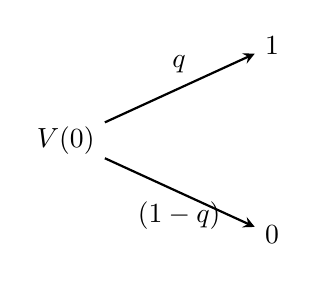
\begin{tikzpicture}[>=stealth, thick,scale=1.2]
			\node (A1) at (0,0) {$V(0)$};
			\node (B1) at (2,1) [right]{$1$};
			\node (C1) at (2,-1) [right]{$0$};
			\draw [->](A1)--(B1); \draw [->](A1)--(C1);
			\node at (1.2,.8){$q$};  \node at (1.2,-.8){$(1-q)$};  
			%\node at (0,-1.8){$t=0$};
			%\node at (2.5,-1.8){$t=1$};
		\end{tikzpicture}
	\end{center}

	由于期权剩余到期时间仅有三个月,因此在单利计息下,将年利率的1/4作为利息的计算依据。
于是可得:
\[V(0)=\frac{1}{1+4\%/4}\left[q\cdot  1+(1-q)\cdot 0\right]=\frac{0.55}{1+4\%/4}=0.545 \]

\end{frame}

\begin{frame}{例题2:看跌期权}
	一只股票的当前价格为20元,三个月后股价有可能涨至22元,也有可能跌至18元。该股票三个月后到期的看跌期权的行权价为21元,假设无风险利率为4\%。

问:该看跌期权的当前价格应为多少?
\end{frame}

\begin{frame}{解答}
	此处要求的是看跌期权的价格,其他条件与前例完全相同,因此
$u=22/20=1.1,\; d=18/20=0.9,\; K=21$。
\begin{center}
	\begin{tikzpicture}[>=stealth, thick,scale=0.8]
		\node (A) at (0,0) {$20$};
		\node (B) at (2.5,1) {$22$};
		\node (C) at (2.5,-1) {$18$};
		\draw [->](A)  to (B)  ; \draw [->](A)--(C);
		\node at (1,.8){$q$};  \node at (1,-.8){$(1-q)$};  
		%\node at (0,-1.8){$t=0$};
		%\node at (2.5,-1.8){$t=1$};
		
		\node at (1.5, -1.8) {(a)股票的二叉树};
		\end{tikzpicture}\qquad 
		\begin{tikzpicture}[>=stealth, thick,scale=0.8]
		\node (A1) at (0,0) {$V(0)$};
		\node (B1) at (2,1) [right]{$\max(0, 21-22)=0$};
		\node (C1) at (2,-1) [right]{$\max(0, 21-18)=3$};
		\draw [->](A1)--(B1); \draw [->](A1)--(C1);
		\node at (1.2,.8){$q$};  \node at (1.2,-.8){$(1-q)$};  
		%\node at (0,-1.8){$t=0$};
		%\node at (2.5,-1.8){$t=1$};
		\node at (2, -1.8){(b)期权的二叉树};
		\end{tikzpicture}
\end{center}

于是可得:
\[V(0)=\frac{1}{1+4\%/4}\left[q\cdot  0+(1-q)\cdot 3\right]=\frac{0.45\times 3}{1+1\%}=1.337  \]
\end{frame}

\section{多期二项式模型}
\begin{frame}{多期二项式模型}
	二项式模型所得的结果尽可能地符合或接近实际,只需要将标的资产价格变动的期间(period)增加到两个或两个以上,从而使单期二项式模型变为多期二项式模型(multi-period binomial model)。

	假设标的股票的当前价格为$S$,无风险利率为$r$,每期的时间跨度为$1$;未来每期结束时,价格有两种可能的变化:要么上涨至原来的$u$ 倍($u>1$),要么下跌至原来的$d$倍($0<d<1$)。根据这一假设可以画出该股票对应的二叉树。
\begin{center}
	\begin{tikzpicture}[>=stealth, thick, scale=.9]

		\node (A) at (0,0) {$S$};
		\node (B1) at (1.5,0.5) {$uS$};
		\node (B2) at (1.5,-0.5) {$dS$};
		\node (C1) at (3.5,1) {$uuS$};
		\node (C2) at (3.5,0) {$udS$};
		\node (C3) at (3.5,-1) {$ddS$};
		\draw [->] (A)--(B1);
		\draw [->] (A)--(B2);
		\draw [->] (B1)--(C1);
		\draw [->] (B1)--(C2);
		\draw [->] (B2)--(C2);
		\draw [->] (B2)--(C3);
		\node at (0,-1.5){当前};
		\node at (1.5,-1.5){第1期};
		\node at (3.5,-1.5){第2期};
		
		\end{tikzpicture}
\end{center}
\end{frame}

\begin{frame}{多期二项式模型的风险中性概率}
	由于风险中性概率$q$ 只与无风险利率$r$ 、时间跨度$t=1$ 、上涨倍数$u$ 和下跌倍数$d$ 有关,而与股票的价格$S$ 无关,即:
	 \[q=\frac{(1+r)-d}{u-d} \]
因此,风险中性概率可以应用于整个二叉树的各个分支。

\begin{block}{注意:}
	金融中通常使用连续复利计息法,于是上面的风险中性概率计算公式相应地改写为:
\begin{equation*}
q=\frac{{\rm e}^{rt}-d}{u-d}
\end{equation*}
其中,$r$是无风险利率,$t$是各期之间的时间跨度。在后面所述的多期二项式模型定价中,将使用上式计算风险中性概率。
\end{block}
\end{frame}

\subsection{欧式期权的定价}
\begin{frame}{例题3:}
	假设标的股票的当前价格为100元,每期的时间跨度为1年。未来每年结束时,价格有两种可能的变化:要么上涨至原来的1.1倍,要么下跌至原来的0.9倍。当前距离期权到期还有两期,已知每期的无风险利率均为5\%。求:
\begin{enumerate}[(1)]
\item 行权价为105元的欧式看涨期权的当前价格。
\item 行权价为105元的欧式看跌期权的当前价格。
\end{enumerate}
\end{frame}

\begin{frame}{解答}
	\begin{center}
\begin{tikzpicture}[>=stealth, thick, scale=1.3]

\node (A) at (0,0) {$100$};
\node (B1) at (1.5,0.5) {$110$};
\node (B2) at (1.5,-0.5) {$90$};
\node (C1) at (3.5,1) {$121$};
\node (C2) at (3.5,0) {$99$};
\node (C3) at (3.5,-1) {$81$};

\node at (.75,.5){$q$};  \node at (.75,-.6){$(1-q)$};
\node at (2.5,.9){$q$};    \node at (2.5,0){$(1-q)$};
\node at (2.5,-.4){$q$};    \node at (2.5,-1){$(1-q)$};
\draw [->] (A)--(B1);
\draw [->] (A)--(B2);
\draw [->] (B1)--(C1);
\draw [->] (B1)--(C2);
\draw [->] (B2)--(C2);
\draw [->] (B2)--(C3);
\node at (0,-1.5){当前};
\node at (1.5,-1.5){第1期};
\node at (3.5,-1.5){第2期};

\end{tikzpicture}		
	\end{center}

	已知$u=1.1,\; d=0.9,\; K=105,\; r=5\%,\; t=1$,可以计算得到风险中性概率$q$: 
	 	 \[q=\frac{{\rm e}^{rt}-d}{u-d}=\frac{{\rm e}^{5\%}-0.9}{1.1-0.9}=0.756 \]
\end{frame}

\begin{frame}{解答:看涨期权的二叉树}\small
	\begin{center}
\begin{tikzpicture}[>=stealth, thick, scale=1.2]

\node (A) at (0,0) {$C_0$};
\node (B1) at (1.5,0.5) {$C_{11}$};
\node (B2) at (1.5,-0.5) {$C_{12}$};
\node (C1) at (3.5,1) {$16$};
\node (C2) at (3.5,0) {$0$};
\node (C3) at (3.5,-1) {$0$};

\node at (.75,.5){$q$};  \node at (.75,-.6){$(1-q)$};
\node at (2.5,.9){$q$};    \node at (2.5,0){$(1-q)$};
\node at (2.5,-.4){$q$};    \node at (2.5,-1){$(1-q)$};
\draw [->] (A)--(B1);
\draw [->] (A)--(B2);
\draw [->] (B1)--(C1);
\draw [->] (B1)--(C2);
\draw [->] (B2)--(C2);
\draw [->] (B2)--(C3);
\node at (0,-1.5){当前};
\node at (1.5,-1.5){第1期};
\node at (3.5,-1.5){第2期};

\end{tikzpicture}
	\end{center}

	由此可得:
	\[\begin{split}
	C_{11}&={\rm e}^{-rt}[q\cdot 16+(1-q)\cdot 0]={\rm e}^{-5\%}(0.756\times 16)=11.51  \\
	C_{12}&={\rm e}^{-rt}[q\cdot 0+(1-q)\cdot 0]=0
	\end{split} \]
	最终:
	\[C_0={\rm e}^{-rt}[q\cdot C_{11}+(1-q)\cdot C_{12}]={\rm e}^{-5\%}(0.756\times 11.43)=8.27 \]

\end{frame}

\begin{frame}{解答:看跌期权的二叉树}\small
	\begin{center}
		\begin{tikzpicture}[>=stealth, thick, scale=1.2]

			\node (A) at (0,0) {$P_0$};
			\node (B1) at (1.5,0.5) {$P_{11}$};
			\node (B2) at (1.5,-0.5) {$P_{12}$};
			\node (C1) at (3.5,1) {$0$};
			\node (C2) at (3.5,0) {$6$};
			\node (C3) at (3.5,-1) {$24$};
			
			\node at (.75,.5){$q$};  \node at (.75,-.6){$(1-q)$};
			\node at (2.5,.9){$q$};    \node at (2.5,0){$(1-q)$};
			\node at (2.5,-.4){$q$};    \node at (2.5,-1){$(1-q)$};
			\draw [->] (A)--(B1);
			\draw [->] (A)--(B2);
			\draw [->] (B1)--(C1);
			\draw [->] (B1)--(C2);
			\draw [->] (B2)--(C2);
			\draw [->] (B2)--(C3);
			\node at (0,-1.5){当前};
			\node at (1.5,-1.5){第1期};
			\node at (3.5,-1.5){第2期};
			
			\end{tikzpicture}
	\end{center}

	由此可得:
\[\begin{split}
 P_{11}&={\rm e}^{-rt}[q\cdot 0+(1-q)\cdot 6]={\rm e}^{-5\%}(0.244\times 11)=1.39  \\
P_{12}&={\rm e}^{-rt}[q\cdot 6+(1-q)\cdot 24]={\rm e}^{-5\%}(0.756\times 11+0.25\times 29)=9.89
\end{split} \]
最终:
\[\begin{split}
    P_0&={\rm e}^{-rt}[q\cdot P_{11}+(1-q)\cdot P_{12}]\\
    &={\rm e}^{-5\%}(0.756\times 1.39+0.244\times 9.89)=3.3
\end{split}\]
\end{frame}

\begin{frame}{归纳}
	假设期权的剩余期限为$T$,将期权的期间数分为$n$个相等的时间段$\Delta t$,因此$\Delta t=T/n$。
由于在$n$次二项步骤后,$i$次上涨和$(n-i)$次下跌的风险中性概率为:
\[\Pr(\#u=i,\;\#d=n-i)={n\choose i}q^i(1-q)^{n-i} =\frac{n!}{i!(n-i)!}q^i(1-q)^{n-i}\]
其中,$\#u$和$\#d$分别表示期权的剩余期限内,资产价格上涨和下跌的总次数。
对应的看涨期权回报数额为:
\[\max\left(S_0 u^id^{n-i}-K,0\right) \]
\end{frame}

\begin{frame}{归纳(cont.)}\small
$n$期二项式模型当中,欧式看涨期权的定价公式为:
\begin{equation*}
\begin{split}
C_0&= {\rm e}^{-rn\Delta t}\Pr(\#u=i,\;\#d=n-i)\cdot \max\left(S_0 u^id^{n-i}-K,0\right)\\
&={\rm e}^{-rT}\sum^n_{i=0}{n\choose i}q^i(1-q)^{n-i}\cdot \max\left(S_0 u^id^{n-i}-K,0\right)
\end{split}
\end{equation*} 
其中:
\[q=\frac{{\rm e}^{r\Delta t}-d}{u-d}\]

类似地,欧式看跌期权的定价公式为:
\begin{equation*}
\begin{split}
P_0&= {\rm e}^{-rn\Delta t}\Pr(\#u=i,\;\#d=n-i)\cdot \max\left(K-S_0 u^id^{n-i},0\right)\\
&={\rm e}^{-rT}\sum^n_{i=0}{n\choose i}q^i(1-q)^{n-i}\cdot \max\left(K-S_0 u^id^{n-i},0\right)
\end{split} 
\end{equation*}
\end{frame}

\subsection{美式期权的定价}
\begin{frame}{美式期权的定价}
	二项式模型不仅可以给欧式期权进行定价,还可以给美式期权、奇异期权等进行定价。与欧式期权不同,美式期权在到期前的任何一天均可以提前行权。这一特征使得美式期权的定价问题比欧式期权要复杂。

在二项式模型当中,对美式期权进行定价时,需要考虑期权提前行权的收益与期权价值之间的差异,然后取两者中的较大者作为下一期计算的节点数值。
\end{frame}

\begin{frame}{例题4:}
	假设标的股票的当前价格为100,未来每期结束时,价格有两种可能的变化:要么上涨至原来的1.5倍,要么下跌至原来的0.75倍。当前距离期权到期还有两期,已知每期的无风险利率均为5\%。

求行权价为110的美式看涨期权的当前价格。
\end{frame}

\begin{frame}{解答}
	已知:$u=1.5$,$d=0.75$,$K=110$,$r=5\%$。可以计算得到风险中性概率$q$:
\[q=\frac{{\rm e}^{rt}-d}{u-d}=\frac{{\rm e}^{5\%}-0.75}{1.5-0.75}=0.402  \]

首先构造股票价格的二叉树,同时计算出各期看涨期权的可能价值,计算结果反映在括号内。
\begin{center}
	\begin{tikzpicture}[>=stealth, thick, scale=1.3]  
		\node (A) at (-1,0) {$100(0)$};
		\node (B1) at (1.5,0.5) {$150(40)$};
		\node (B2) at (1.5,-0.5) {$75(0)$};
		\node (C1) at (4.5,1) {$225(115)$};
		\node (C2) at (4.5,0) {$112.5(2.5)$};
		\node (C3) at (4.5,-1) {$56.25(0)$};
		\node at (.5,.5){$q$};  \node at (.5,-.6){$(1-q)$};
		\node at (3,.9){$q$};    \node at (3,0){$(1-q)$};
		\node at (3,-.4){$q$};    \node at (3,-1){$(1-q)$};
		\draw [->] (A)--(B1);
		\draw [->] (A)--(B2);
		\draw [->] (B1)--(C1);
		\draw [->] (B1)--(C2);
		\draw [->] (B2)--(C2);
		\draw [->] (B2)--(C3);
		\node at (-1,-1.5){当前};
		\node at (1.5,-1.5){第1期};
		\node at (4.5,-1.5){第2期};
		\end{tikzpicture}
\end{center}
\end{frame}

\begin{frame}{解答(cont.)}
接下来,使用风险中性概率,结合第2期看涨期权的可能价值,计算出第1期期权的价值分别为:
\[\begin{split}
c_1&={\rm e}^{-5\%}[0.402\times 115+(1-0.402)\times 2.5] =45.4\\
c_2&={\rm e}^{-5\%}[0.402\times 2.5+(1-0.402)\times 0]=0.96 \\
\end{split} \]
由于美式期权可在到期日之前的任意时刻行权,因此需要将求得的结果与第1期美式期权的价值进行比较,并取较大者,所以:
\[\begin{split}
c_{11}&=\max(45.4, 40)=45.4\\
c_{12}&=\max(0.96, 0)=0.96\\
\end{split} \]
\end{frame}

\begin{frame}{解答(cont.)}
	最后,使用求得的第1期期权的价值$c_{11}$和$c_{12}$,计算出当前期权的价格:
\[c_0=\max\left\{0, {\rm e}^{-5\%} [0.402\times 45.4+(1-0.402)\times 0.96] \right\}=17.91 \]

\begin{center}
		\begin{tikzpicture}[>=stealth, thick, scale=1.4]

			\node (A) at (-.5,0) {$17.91$};
			\node (B1) at (1.5,0.5) {$45.4$};
			\node (B2) at (1.5,-0.5) {$0.96$};
			\node (C1) at (3.5,1) {$115$};
			\node (C2) at (3.5,0) {$2.5$};
			\node (C3) at (3.5,-1) {$0$};
			
			\node at (.5,.5){$q$};  \node at (.5,-.6){$(1-q)$};
			\node at (2.5,.9){$q$};    \node at (2.5,0){$(1-q)$};
			\node at (2.5,-.4){$q$};    \node at (2.5,-1){$(1-q)$};
			\draw [->] (A)--(B1);
			\draw [->] (A)--(B2);
			\draw [->] (B1)--(C1);
			\draw [->] (B1)--(C2);
			\draw [->] (B2)--(C2);
			\draw [->] (B2)--(C3);
			\node at (-.5,-1.5){当前};
			\node at (1.5,-1.5){第1期};
			\node at (3.5,-1.5){第2期};
			
			\end{tikzpicture}
\end{center}
\end{frame}

\subsection{障碍期权的定价}
\begin{frame}{障碍期权的定价举例}
	假设标的股票的当前价格为100,未来每期结束时,价格有两种可能的变化:要么上涨至原来的1.1倍,要么下跌至原来的0.9倍。当前距离期权到期还有三期,已知每期的无风险利率均为5\%。

	求行权价为105、障碍敲出价格为95的看涨期权的当前价格。	

	\begin{block}{思路:}
		由于障碍期权可以提前中止,所以使用二项式模型进行定价时,需要关注标的资产二叉树的各节点与障碍价格之间的关系。
	\end{block}
\end{frame}

\begin{frame}{解答}
	首先绘制出该期权的对应标的股票价格的二叉树,图中的虚线位置对应的是期权的障碍价格95,当标的资产的价格低于此值时,期权自动作废,对应的期权二叉树的相应节点取值为零。
	\begin{center}
        \begin{tikzpicture}[>=stealth, thick, scale=1]
        
        \node (A) at (0,0) {$100$};
        \node (B1) at (1.5,0.5) {$110$};
        \node (B2) at (1.5,-0.5) {$90$};
        \node (C1) at (3.5,1) {$121$};
        \node (C2) at (3.5,0) {$99$};
        \node (C3) at (3.5,-1) {$81$};
        \node (D1) at (5.5,1.5) {$133.1$};
        \node (D2) at (5.5,0.5) {$108.9$};
        \node (D3) at (5.5,-.5) {$89.1$};
        \node (D4) at (5.5,-1.5) {$72.9$};
  
        \draw [->] (A)--(B1);
        \draw [->] (A)--(B2);
        \draw [->] (B1)--(C1);
        \draw [->] (B1)--(C2);
        \draw [->] (B2)--(C2);
        \draw [->] (B2)--(C3);
        \draw [->] (C1)--(D1);
        \draw [->] (C1)--(D2);
        \draw [->] (C2)--(D2);
        \draw [->] (C2)--(D3);
        \draw [->] (C3)--(D3);
        \draw [->] (C3)--(D4);
        
        \node at (0,-2){当前};
        \node at (1.5,-2){第1期};
        \node at (3.5,-2){第2期};
        \node at (5.5,-2){第3期};
        
        \draw[dashed](-.25,-.2)--(6,-.2);
        \end{tikzpicture} 
	\end{center}
\end{frame}

\begin{frame}{解答(cont.)}
	风险中性概率计算如下:
\[q = \frac{{{{\rm e}^{rt}} - d}}{{u - d}} = \frac{{{{\rm e}^{5\% }} - 0.9}}{{1.1 - 0.9}} = 0.756\]
	\begin{center}
		\begin{tikzpicture}[>=stealth, thick, scale=1]

            \node (A) at (0,0) {$C_0$};
            \node (B1) at (1.5,0.5) {$C_{11}$};
            \node (B2) at (1.5,-0.5) {$0$};
            \node (C1) at (3.5,1) {$C_{21}$};
            \node (C2) at (3.5,0) {$C_{22}$};
            \node (C3) at (3.5,-1) {$0$};
            \node (D1) at (5.5,1.5) {$28.1$};
            \node (D2) at (5.5,0.5) {$3.9$};
            \node (D3) at (5.5,-.5) {$0$};
            \node (D4) at (5.5,-1.5) {$0$};
            \draw [->] (A)--(B1);
            \draw [->] (A)--(B2);
            \draw [->] (B1)--(C1);
            \draw [->] (B1)--(C2);
            \draw [->] (B2)--(C2);
            \draw [->] (B2)--(C3);
            \draw [->] (C1)--(D1);
            \draw [->] (C1)--(D2);
            \draw [->] (C2)--(D2);
            \draw [->] (C2)--(D3);
            \draw [->] (C3)--(D3);
            \draw [->] (C3)--(D4);
            
            \node at (0,-2){当前};
            \node at (1.5,-2){第1期};
            \node at (3.5,-2){第2期};
            \node at (5.5,-2){第3期};
            
            \draw[dashed](-.25,-.2)--(6,-.2);
            \end{tikzpicture}
	\end{center}
\end{frame}

\begin{frame}{解答(cont.)}\small
	\begin{center}
		\begin{tikzpicture}[>=stealth, thick, scale=.85]
            \node (A) at (0,0) {$C_0$};
            \node (B1) at (1.5,0.5) {$C_{11}$};
            \node (B2) at (1.5,-0.5) {$0$};
            \node (C1) at (3.5,1) {$C_{21}$};
            \node (C2) at (3.5,0) {$C_{22}$};
            \node (C3) at (3.5,-1) {$0$};
            \node (D1) at (5.5,1.5) {$28.1$};
            \node (D2) at (5.5,0.5) {$3.9$};
            \node (D3) at (5.5,-.5) {$0$};
            \node (D4) at (5.5,-1.5) {$0$};
            \draw [->] (A)--(B1);
            \draw [->] (A)--(B2);
            \draw [->] (B1)--(C1);
            \draw [->] (B1)--(C2);
            \draw [->] (B2)--(C2);
            \draw [->] (B2)--(C3);
            \draw [->] (C1)--(D1);
            \draw [->] (C1)--(D2);
            \draw [->] (C2)--(D2);
            \draw [->] (C2)--(D3);
            \draw [->] (C3)--(D3);
            \draw [->] (C3)--(D4);
            
            \node at (0,-2){当前};
            \node at (1.5,-2){第1期};
            \node at (3.5,-2){第2期};
            \node at (5.5,-2){第3期};
            
            \draw[dashed](-.25,-.2)--(6,-.2);
            \end{tikzpicture}
	\end{center}
	接下来使用后向推导法,依次计算出各期的期权价值,结果如下:
\[\begin{split}
C_{21} &= {{\rm e}^{ - 5\% }}\left[ {0.756 \times 28.1 + (1 - 0.756) \times 3.9} \right] = 21.12\\
C_{22} &= {{\rm e}^{ - 5\% }}\left[ {0.756 \times 3.9 + (1 - 0.756) \times 0} \right] = 2.806\\
C_{11} &= {{\rm e}^{ - 5\% }}\left[ {0.756 \times 21.12 + (1 - 0.756) \times 2.806} \right] = 15.85\\
C_0 &= {{\rm e}^{ - 5\% }}\left[ {0.756 \times 15.85 + (1 - 0.756) \times 0} \right] = 11.4
\end{split}\]
\end{frame}

\begin{frame}{障碍期权定价的说明}
	这个例题中并未涉及向上/向下敲出这样的复杂情形。
	
	在计算的二叉树期数和路径较少的情况下,该方法是简单易行的,但是如果期数$N$过大,则需要仔细分辨$2^N$条可能路径下期权生效和失效的情形,这将是非常费力的。
\end{frame}


\subsection{其他期权品种的定价简介}
\begin{frame}{连续分红的股票期权定价}
	考虑一只股票,其连续分红的股息收益率为$q^*$。在风险中性测度下,该股票未来时刻价格期望值的贴现应当等于其前一期股票价格关于股息收益率的贴现值,即:
\[{S_0}{{\rm e}^{ - {q^*}t}} = [qu{S_0} + (1 - q)d{S_0}]{{\rm e}^{ - rt}}\]
对上式进行整理可得:
\begin{equation*}
q = \frac{{\exp \left[ {(r - {q^*})t} \right] - d}}{{u - d}}
\end{equation*}
\end{frame}

\begin{frame}{股票指数期权的定价}
	对于由一组股票所构成的股票指数而言,由于股票指数中包含的各成份股具有不同的股息支付日,可以将之近似地看作一个有连续分红的股票组合。对于这样的一个股票组合所对应的期权进行二项式定价,可以沿用下式来计算风险中性概率。
	\begin{equation*}
		q = \frac{{\exp \left[ {(r - {q^*})t} \right] - d}}{{u - d}}
		\end{equation*}
\end{frame}

\begin{frame}{外汇期权的定价}
	外汇期权的标的物是外国货币(即外汇),外汇可以看作获得外币利率$r_f$ 的资产。与前面提到的连续分红的股票期权和股票指数期权相似,仍然可以参照前式来计算风险中性概率。修正后的计算公式如下:
\begin{equation*}
q = \frac{{\exp \left[ {(r - {r_f})t} \right] - d}}{{u - d}}
\end{equation*}
其中,$r$表示本币的无风险利率; $r_f$表示外币的无风险利率,并且此处的外汇汇率采用直接报价法(即一单位外币等于若干单位本币)。
\end{frame}

\begin{frame}{期货期权的定价}
	对于期货期权而言,其标的资产已不再是现货,而是现货所对应的期货合约。由于现货价格$S$ 与期货价格$F$ 之间的关系式为:
\[F=S{\rm e}^{rt} \]
因此,对于期货期权而言,其二项式定价模型当中下式成立:
\[quF_0+(1-q)dF_0=F_0 \]
对上式进行整理可得:
\begin{equation*}
q=\frac{1-d}{u-d}
\end{equation*}
\end{frame}

\begin{frame}{注意事项}
	在实证中根据所采用的模型不同,我们将选择不同的模型公式来计算标的资产价格上涨和下跌的倍数$u$ 和$d$ ,比如CRR模型、JR(Jarrow-Rudd)模型等等。
\end{frame}

\section{CRR模型}
\subsection{CRR模型的设定}
\begin{frame}{CRR模型的设定}
	最早基于二项式模型框架进行期权定价的方法是由考克斯、罗斯和鲁宾斯坦于1979年提出的,因此被命名为CRR模型。在CRR模型中,假定标的资产的波动率为$\sigma$,每个时间段为$\Delta t$,则标的资产上涨的倍数$u$与下跌的倍数$d$之间具有如下关系:
\begin{equation*}
u=\frac{1}{d},\qquad \begin{cases}
\vspace{1ex} u=\exp\left(\sigma\sqrt{\Delta t}\right)\\
d=\exp\left(-\sigma\sqrt{\Delta t}\right) \\
\end{cases}
\end{equation*}
相应地,风险中性概率为:
\begin{equation*}
q=\frac{{\rm e}^{r\Delta t}-d}{u-d}=\frac{{\rm e}^{r\Delta t}-{\rm e}^{-\sigma\sqrt{\Delta t}}}{{\rm e}^{\sigma\sqrt{\Delta t}}-{\rm e}^{-\sigma\sqrt{\Delta t}}}
\end{equation*}
\end{frame}

\begin{frame}{CRR模型(cont.)}
	基于CRR模型,假设$n$期的二叉树,相应的期权剩余期限为$T=n\Delta t$,于是
可以得到对应的欧式期权定价公式如下:
\begin{equation*}\small
\begin{split}
C_0&={\rm e}^{-rT}\sum^n_{i=0}{n\choose i}q^i(1-q)^{n-i}\cdot \max\left(S_0 u^id^{n-i}-K,0\right)\\
&={\rm e}^{-rT}\sum^n_{i=0}{n\choose i}q^i(1-q)^{n-i}\cdot \max\left\{S_0 \exp\left[(2i-n)\sigma\sqrt{\Delta t} \right] -K,0\right\}\\
\end{split}
\end{equation*}
\begin{equation*}\small
\begin{split}
P_0&={\rm e}^{-rT}\sum^n_{i=0}{n\choose i}q^i(1-q)^{n-i}\cdot \max\left(K-S_0 u^id^{n-i},0\right)\\
&={\rm e}^{-rT}\sum^n_{i=0}{n\choose i}q^i(1-q)^{n-i}\cdot \max\left\{K-S_0\exp \left[(2i-n)\sigma\sqrt{\Delta t} \right],0\right\}
\end{split}
\end{equation*}
\end{frame}

\subsection{CRR模型与B-S模型的联系}
\begin{frame}{CRR模型与B-S模型的对比}
	\centering
	\includegraphics[scale=.7]{fig/Bino-BS.PDF}
\end{frame}

\end{document}

